\documentclass[11pt, oneside]{article}
\usepackage[margin=1in,letterpaper]{geometry}
\usepackage{times}
\usepackage{graphicx}
\usepackage{amssymb,amsmath,mathtools}
\usepackage{array}
\usepackage{longtable}
\usepackage{color}
\usepackage[T1]{fontenc}
\usepackage{sectsty}
\usepackage[normalem]{ulem}
\usepackage{tikz}
\usetikzlibrary{decorations.pathmorphing,calc,arrows.meta,patterns}
\usepackage{pgfplots}
\pgfplotsset{compat=1.17}
\usepackage{float}
\sectionfont{\fontsize{12}{12}\selectfont}
\subsectionfont{\fontsize{11}{11}\selectfont}
\subsubsectionfont{\normalsize\itshape\mdseries}

\renewcommand\labelitemi{{\boldmath$\cdot$}}
\renewcommand\labelitemii{\labelitemi}
\renewcommand\labelitemiii{\labelitemi}
\renewcommand\labelitemiv{\labelitemi}

%%%%%%%%%%%%%%%%%%%%%%%%%%%%%%%%%%%%%
% NOTE: Lecture 15 is new (drafted 2026-11-19 at the instructor's request): an optional module on the physics behind
% InSAR measurements, for students who will meet InSAR as a geodetic tool in Tectonic Geodesy. There are no
% handwritten notes; the content is written from the references below, in the style of Lectures 7-14, and every
% equation was checked by derivation and python3 numerics (scratchpad l15_checks.py).
% Notation: symbols follow ../variables_master.tex. It continues Lecture 14: the phase of a focused SAR pixel is
% phi = -4 pi R/lambda (L14, Eq. e:phis), with the e^{j omega t} convention. New dual usages are flagged in the master
% table (D166-D174, all approved 2026-11-19). Choices made to avoid new clashes:
%   - complex pixel values V_1, V_2 (extends L14's compressed signal V_o; van Zyl 2011 writes V_1 V_2^*, Eq. 3.5-9);
%   - baseline components B_par, B_perp only (no baseline angle alpha, which is the attenuation constant);
%   - partial pressures P_dry, P_vap (Hanssen's P_d and e; e is the elementary charge and emissivity);
%   - gas constants written R_gas/M and R_gas/M_vap (no R_d, R_v; R is range);
%   - excess path lengths written Delta R_atm, Delta R_hyd, Delta R_wet, Delta R_iono (L is taken several times);
%   - the chirp bandwidth B of L14 is not used (B is the baseline here); the band of wavenumbers is written with X_r;
%   - theta: look angle (L14); on a flat Earth without topography theta_i = theta (L14, Fig. 2 caption), so theta is
%     used throughout, including in the L8 Bragg wavenumber and the L9 canopy factor;
%   - rms scatterer displacements Delta y_rms, Delta z_rms (Zebker & Villasenor: sigma_y, sigma_z; sigma is taken);
%   - standard deviation of the phase written std(Delta phi) (no new sigma);
%   - the ionospheric constant written as e^2/(8 pi^2 eps_0 m_e) = 40.3 m^3/s^2 (no K, which is taken).
% Interferogram convention (as in van Zyl 2011, Eqs. 3.5-2 and 3.5-9): V_1 V_2^*, Delta phi = phi_1 - phi_2, with
% image 1 the first (reference) acquisition in repeat-pass interferometry.
%%%%%%%%%%%%%%%%%%%%%%%%%%%%%%%%%%%%%

\newcommand{\Bperp}{B_\perp}
\newcommand{\Bpar}{B_\parallel}
\newcommand{\Bc}{B_{\perp,\mathrm{c}}}
\newcommand{\zamb}{z_{2\pi}}
\newcommand{\Nlooks}{N_\mathrm{looks}}
\newcommand{\wv}{\mathrm{w_{vap}}}
\newcommand{\Pvap}{P_\mathrm{vap}}
\newcommand{\Pdry}{P_\mathrm{dry}}
\newcommand{\Mvap}{M_\mathrm{vap}}
\newcommand{\TEC}{\mathrm{TEC}}
\newcommand{\gt}{\tilde{\gamma}}

\title{Ge 158 Lecture 15: The Physics of InSAR Measurements}
\author{Brent Minchew}
\date{}

\setlength{\emergencystretch}{1.5em}
\renewcommand{\topfraction}{0.85}
\renewcommand{\textfraction}{0.1}
\renewcommand{\floatpagefraction}{0.75}
\begin{document}
\maketitle

\noindent\underline{\textbf{Topics covered}}
\begin{itemize}
	\item The phase of a SAR pixel and the interferogram
	\item What the interferometric phase measures: topography, deformation, and everything else
	\item Coherence and the physics of decorrelation
	\item Propagation delays in the troposphere and ionosphere
	\item Choosing a wavelength
\end{itemize}

\noindent This is an optional module. Interferometric SAR (InSAR) as a geodetic tool, including phase unwrapping, time series, and modeling of deformation sources, is covered in Tectonic Geodesy. Here we focus on the physics that sets what InSAR can measure, building on the scattering (Lectures 7--9), atmosphere (Lectures 10--11), and SAR (Lecture 14) lectures.

%%%%%%%%%%%%%%%%%%%%%%%%%%%%%%%%%%%%%
\section{From SAR images to interferograms}
\label{s:interferogram}

\subsection{The phase of a SAR pixel}

\begin{itemize}
	% NOTE: L14, Eq. (e:phis): phi(s) = -4 pi R(s)/lambda; after azimuth compression the phase of a point scatterer is
	% that at closest approach, -4 pi R_0/lambda (van Zyl 2011, Sec. 1.5, pp. 14-15).
	\item In Lecture 14, we found that after range compression the signal from a point scatterer carries the phase $\phi(s) = -4\pi R(s)/\lambda$ (Lecture 14, Eq.~17; the carrier $e^{j\omega_0t}$ is removed when the received signal is demodulated). Azimuth compression removes the quadratic (Doppler) part of $\phi(s)$ and leaves the phase at closest approach, so the focused pixel has phase
	\begin{equation}
		\label{e:phi}
		\phi = -\frac{4\pi R_0}{\lambda} \equiv -\frac{4\pi R}{\lambda}
	\end{equation}
	where from here on we drop the subscript and write $R$ for the range at closest approach. The factor $4\pi$ (rather than $2\pi$) is because the wave travels to the scatterer and back.
	\item A pixel, however, is not a point scatterer. A resolution cell ($X_r \times X_a^\mathrm{SAR}$, meters to tens of meters for modern systems) contains many scatterers (soil grains, rocks, leaves, branches), and the focused pixel value is the coherent sum of their echoes:
	\begin{equation}
		\label{e:Vpixel}
		V = \sum_n E_{r(n)}\,e^{-j4\pi R_{(n)}/\lambda} = |V|e^{j\phi}
	\end{equation}
	where $E_{r(n)}$ is the (complex) field received from scatterer $n$ (the $E_r$ of Lecture 14) and $R_{(n)}$ is its range.
	% NOTE: the sinc weighting of the point-target response (L14, Eq. e:Vo) is absorbed into E_r(n).
	\item The ranges $R_{(n)}$ differ by many wavelengths across a resolution cell, so the phases of the terms are effectively random, and so is their sum
	\begin{itemize}
		\item[$\Rightarrow$] The phase $\phi$ of a single SAR image is uniformly distributed on $(-\pi, \pi]$ from pixel to pixel and tells us nothing by itself
		\item[$\Rightarrow$] The amplitude $|V|$ fluctuates strongly from pixel to pixel, even over a uniform surface: this is \emph{speckle}
		% NOTE: for many independent scatterers, Re V and Im V are zero-mean Gaussian (central limit theorem), so |V| is
		% Rayleigh distributed and phi is uniform (Goodman's fully developed speckle; Hanssen 2001, Sec. 4.2).
	\end{itemize}
\end{itemize}

\subsection{The interferogram}

\begin{itemize}
	\item Now suppose we image the same resolution cell twice, from almost the same position, and the scatterers have not changed. Then each term in Eq.~\eqref{e:Vpixel} is the same in both images except for a change in range
	\item If every scatterer in the cell moves by the same amount, so that $R_{(n)} \to R_{(n)} + \Delta R$, then $V_2 = V_1e^{-j4\pi\Delta R/\lambda}$
	\item The \emph{interferogram} is the product of one image with the complex conjugate of the other,
	\begin{equation}
		\label{e:ifg}
		V_1V_2^* = |V_1||V_2|\,e^{j(\phi_1 - \phi_2)} \qquad\Rightarrow\qquad \Delta\phi \equiv \phi_1 - \phi_2 = \frac{4\pi\,\Delta R}{\lambda} \quad (\mathrm{mod}\ 2\pi)
	\end{equation}
	% NOTE: van Zyl 2011, Eqs. 3.5-1, 3.5-2 and 3.5-9 (pp. 135-138), uses the same order, E(A_1) E(A_2)^* and V_1 V_2^*.
	% Zebker and Villasenor (1992), Eq. 12, Rosen et al. (2000), and Simons and Rosen (2007), Eqs. 13-15, form s_1 s_2^*
	% with phi = -4 pi r/lambda, as here (Simons and Rosen's Eq. 14 has a sign typo, e^{-j...}; their Eq. 15 is right).
	\item The random part of the phase, the arrangement of the scatterers within the cell, is the same in both images and cancels. What remains is the change in range, measured as a fraction of the wavelength
	\begin{itemize}
		\item[$\bigstar$] One cycle of interferometric phase ($2\pi$, a ``fringe'') corresponds to a change in range of $\lambda/2$: 2.8~cm for Sentinel-1 (C-band, $\lambda = 5.55$~cm) and 11.9~cm for NISAR (L-band, $\lambda = 23.8$~cm)
	\end{itemize}
	\item The phase is known only modulo $2\pi$ (it is \emph{wrapped}). Recovering the integer number of cycles, \emph{phase unwrapping}, is covered in Tectonic Geodesy
	\item Everything that follows comes from asking two questions
	\begin{enumerate}
		\item What, besides motion of the surface, changes the range, $\Delta R$? (Section~\ref{s:phase}, Section~\ref{s:delay})
		\item When does the random part of the phase \emph{not} cancel? (Section~\ref{s:coherence})
	\end{enumerate}
\end{itemize}

%%%%%%%%%%%%%%%%%%%%%%%%%%%%%%%%%%%%%
\section{What the interferometric phase measures}
\label{s:phase}

\subsection{Geometry}

\begin{itemize}
	\item In repeat-pass interferometry, the satellite images the same area on two orbits that are separated by a \emph{baseline} $B$, typically tens to hundreds of meters, at times $t_1$ and $t_2$ (days to years apart) (Figure~\ref{f:geom})
	\item Single-pass interferometers (two antennas on one platform, e.g., SRTM; or two satellites flying in formation, e.g., TanDEM-X) image both ends of the baseline at the same time, so nothing on the ground changes between images; if only one antenna transmits, the factor $4\pi$ below becomes $2\pi$ (van Zyl 2011, Eq.~3.5-5)
	\item Decompose the baseline vector (from antenna 1 to antenna 2) into components parallel ($\Bpar$) and perpendicular ($\Bperp$) to the look direction
	% NOTE: van Zyl 2011, Eq. 3.5-4 (p. 137): delta R = R_2 - R_1 ~= -B sin(theta - alpha), with alpha the baseline angle
	% from horizontal, so B_par = B sin(theta - alpha) and B_perp = B cos(theta - alpha); valid for R >> B.
	\item Because $R \gg B$ (hundreds of km vs.\ hundreds of m), the two rays to a point are nearly parallel, and the difference in range is just the projection of the baseline onto the look direction (van Zyl 2011, Eq.~3.5-4):
	\begin{equation}
		\label{e:dRB}
		R_2 - R_1 \approx -\Bpar
	\end{equation}
\end{itemize}

\begin{figure}[!htbp]
	\centering
	% NOTE: new sketch, after van Zyl 2011, Fig. 3-32 (p. 136), with the baseline decomposed into B_par and B_perp
	% relative to the look direction. Not to scale (B << R).
	\begin{tikzpicture}[scale=1.0, >={Stealth[length=2.2mm]}]
		% ground and reference surface
		\draw[thick] (-0.5,0) -- (9.5,0);
		\node[below] at (9.2,0) {reference surface ($z = 0$)};
		\draw[thick, decorate, decoration={random steps, segment length=6pt, amplitude=1.5pt}]
			(4.3,0) -- (5.4,0.6) -- (6.4,1.25) -- (7.3,0.7) -- (8.4,0.15);
		% antennas (baseline exaggerated)
		\coordinate (A1) at (0,6);
		\coordinate (A2) at (1.5,7.1);
		\coordinate (P) at (6.4,1.25);
		\fill (A1) circle (2.2pt) node[left=3pt] {antenna 1 (time $t_1$)};
		\fill (A2) circle (2.2pt) node[left=3pt] {antenna 2 (time $t_2$)};
		\draw[very thick] (A1) -- node[above left=-2pt] {$B$} (A2);
		% look direction and ranges
		\draw[->] (A1) -- node[below left=-2pt, pos=0.55] {$R_1$} (P);
		\draw[->] (A2) -- node[above right=-2pt, pos=0.55] {$R_2$} (P);
		\fill (P) circle (1.8pt);
		\node[above right] at (P) {scatterer at height $z$};
		% vertical and look angle
		\draw[dashed, <->] (A1) -- node[pos=0.62, left] {$h$} (0,0);
		\draw ($(A1)+(0,-1.2)$) arc[start angle=-90, end angle={-90+atan(6.4/4.75)}, radius=1.2];
		\node at ($(A1)+(0.33,-1.55)$) {$\theta$};
		% baseline components: Q is the projection of antenna 2 onto the look direction from antenna 1
		\coordinate (Q) at ($(A1)!(A2)!(P)$);
		\draw[->, blue!70!black, thick] (A1) -- (Q);
		\draw[->, red!70!black, thick] (Q) -- (A2);
		\draw ($(Q)!0.22cm!(A1)$) -- ($ ($(Q)!0.22cm!(A1)$) + ($(Q)!0.22cm!(A2)$) - (Q) $) -- ($(Q)!0.22cm!(A2)$);
		\node[blue!70!black] at ($(Q)+(0.42,-0.22)$) {$\Bpar$};
		\node[red!70!black, right=2pt] at ($(Q)!0.5!(A2)$) {$\Bperp$};
		% altitude
		\draw[<->] (6.9,0) -- node[right] {$z$} (6.9,1.25);
	\end{tikzpicture}
	\caption{Repeat-pass interferometric geometry in the plane perpendicular to the flight direction (not to scale; in practice $B \ll R$). The baseline $B$ between the two antenna positions has components $\Bpar$ along the look direction and $\Bperp$ perpendicular to it. The difference in range to a scatterer is $R_2 - R_1 \approx -\Bpar$, and $\Bpar$ changes with the look angle $\theta$ at a rate $\Bperp$. After van Zyl (2011), Fig.~3-32.}
	\label{f:geom}
\end{figure}

\subsection{Flat Earth and topography}

\begin{itemize}
	\item $\Bpar$ depends on the look angle: rotating the look direction by $\delta\theta$ changes $\Bpar$ by $\Bperp\,\delta\theta$
	% NOTE: from van Zyl's B_par = B sin(theta - alpha): dB_par/dtheta = B cos(theta - alpha) = B_perp.
	\item So, with Eqs.~\eqref{e:ifg} and \eqref{e:dRB},
	\begin{equation}
		\label{e:dphidtheta}
		\Delta\phi = \frac{4\pi}{\lambda}(R_2 - R_1) = -\frac{4\pi}{\lambda}\Bpar \qquad\Rightarrow\qquad \delta(\Delta\phi) = -\frac{4\pi}{\lambda}\Bperp\,\delta\theta
	\end{equation}
	% NOTE: the sign of Eq. (e:ifg): V_2 = V_1 e^{-j 4 pi (R_2 - R_1)/lambda}, so phi_1 - phi_2 = 4 pi (R_2 - R_1)/lambda;
	% same as van Zyl 2011, Eq. 3.5-5 with a = 2: phi_T = (4 pi/lambda) delta R.
	\item The look angle to a pixel changes for two reasons
	\begin{enumerate}
		\item \emph{Flat Earth}: across the swath, at $z = 0$, $\cos\theta = h/R$, so a step $\delta R$ in range changes the look angle by $\delta\theta = \delta R/(R\tan\theta)$. Even a perfectly flat surface produces fringes, one every
		\begin{equation}
			\label{e:flat}
			\delta R_{2\pi} = \frac{\lambda R\tan\theta}{2\Bperp} \quad\text{in slant range}
		\end{equation}
		% NOTE: python3: Sentinel-1-like values lambda = 5.55 cm, R = 880 km, theta = 37 deg, B_perp = 100 m give 184 m.
		(184~m for Sentinel-1 with $\Bperp = 100$~m). This ``flat-Earth'' phase is computed from the orbits and removed
		\item \emph{Topography}: at a fixed range $R$, a scatterer at height $z$ is seen at a slightly larger look angle than one at $z = 0$, $\delta\theta = z/(R\sin\theta)$
		\begin{equation}
			\label{e:topo}
			\Rightarrow\quad \Delta\phi_\mathrm{topo} = -\frac{4\pi}{\lambda}\frac{\Bperp}{R\sin\theta}\,z
		\end{equation}
		% NOTE: z = h - R cos(theta) at fixed R gives dz = R sin(theta) d theta (van Zyl 2011, Eq. 3.5-6). Same form and
		% sign as Rosen et al. (2000), Eq. 39, and Simons and Rosen (2007), Eqs. 28 and 36, with p = 2; height of
		% ambiguity as Rosen et al. (2000), Eq. 31 (Simons and Rosen define it per radian, 2 pi smaller).
	\end{enumerate}
	\item The \emph{height of ambiguity} is the change in elevation that produces one fringe:
	\begin{equation}
		\label{e:hamb}
		\boxed{\zamb = \frac{\lambda R\sin\theta}{2\Bperp}}
	\end{equation}
	% NOTE: python3: 147 m for Sentinel-1 (lambda = 5.55 cm, R = 880 km, theta = 37 deg) with B_perp = 100 m; 632 m for
	% NISAR L-band with the same geometry.
	\begin{itemize}
		\item For a Sentinel-1-like geometry ($R \approx 880$~km, $\theta \approx 37^\circ$; on the curved Earth the formulas here should use the local incidence angle, which is a few degrees larger than the look angle), $\zamb \approx 150$~m for $\Bperp = 100$~m. For NISAR (L-band) with the same geometry, $\zamb \approx 630$~m
		\item Large $\Bperp$ $\Rightarrow$ high sensitivity to topography (good for making DEMs). Small $\Bperp$ $\Rightarrow$ low sensitivity to topography (good for measuring deformation, because errors in the DEM used to remove $\Delta\phi_\mathrm{topo}$ matter less)
	\end{itemize}
\end{itemize}

\subsection{Deformation and the full phase}

\begin{itemize}
	\item If the ground moves between $t_1$ and $t_2$ so that the range increases by $\Delta R_\mathrm{def}$ (motion away from the radar),
	\begin{equation}
		\label{e:def}
		\Delta\phi_\mathrm{def} = \frac{4\pi}{\lambda}\Delta R_\mathrm{def}
	\end{equation}
	\begin{itemize}
		\item[$\bigstar$] This does not depend on the baseline. Only the component of the displacement along the line of sight is measured
		\item E.g., the first InSAR image of an earthquake (Landers, California, 1992) mapped the displacement around the rupture as fringes; counting fringes and multiplying by $\lambda/2$ gave the line-of-sight displacement field (Massonnet et al., 1993)
		\item[$\bigstar$] A phase measured to $\sim$$0.1$ rad (with averaging; Section~\ref{s:phasenoise}) corresponds to $\Delta R \approx 0.4$~mm at C-band: millimeter-scale sensitivity from an instrument with meter-scale resolution, almost 900~km away
		% NOTE: lambda/(4 pi) * 0.1 rad = 0.44 mm for lambda = 5.55 cm (python3).
	\end{itemize}
	\item In general, the interferometric phase is a sum of several terms:
	\begin{equation}
		\label{e:decomp}
		\Delta\phi = \Delta\phi_\mathrm{flat} + \Delta\phi_\mathrm{topo} + \Delta\phi_\mathrm{def} + \Delta\phi_\mathrm{atm} + \Delta\phi_\mathrm{scat} + \Delta\phi_\mathrm{noise}
	\end{equation}
	% NOTE: Rosen et al. (2000), Eq. 35, and Simons and Rosen (2007), Eq. 32, write phi_obs = phi_topography +
	% phi_displacement; atmosphere and noise are added in their text (Rosen et al. 2000, p. 354; Simons and Rosen 2007,
	% pp. 415-416). The form here combines them.
	\begin{itemize}
		\item[] $\Delta\phi_\mathrm{flat}$, $\Delta\phi_\mathrm{topo}$: geometry (this section); removed using the orbits and a digital elevation model (DEM)
		\item[] $\Delta\phi_\mathrm{def}$: deformation, usually the signal of interest
		\item[] $\Delta\phi_\mathrm{atm}$: different propagation delays through the atmosphere at $t_1$ and $t_2$ (Section~\ref{s:delay})
		\item[] $\Delta\phi_\mathrm{scat}$: change in the phase of the scattering itself, without motion; e.g., a change in soil moisture changes $\varepsilon$ (Lecture 1) and with it the penetration depth (Lecture 2) and the phase of the scattered field, which may produce millimeter-scale apparent range changes (proposed by Nolan et al., 2003)
		\item[] $\Delta\phi_\mathrm{noise}$: random phase from decorrelation (Section~\ref{s:coherence})
	\end{itemize}
\end{itemize}

%%%%%%%%%%%%%%%%%%%%%%%%%%%%%%%%%%%%%
\section{Coherence and decorrelation}
\label{s:coherence}

\subsection{Coherence}

\begin{itemize}
	\item The cancellation in Eq.~\eqref{e:ifg} requires that the scatterers within a resolution cell contribute the same way to both images. When they do not, the interferometric phase acquires a random component, $\Delta\phi_\mathrm{noise}$
	\item The degree to which the two images are alike is measured by the (complex) \emph{coherence}
	\begin{equation}
		\label{e:coh}
		\gt = \frac{\langle V_1V_2^*\rangle}{\sqrt{\langle|V_1|^2\rangle\langle|V_2|^2\rangle}}, \qquad \gamma = |\gt|, \quad 0 \le \gamma \le 1
	\end{equation}
	% NOTE: van Zyl 2011, Eq. 3.5-7 (p. 137); Zebker and Villasenor (1992), Eq. 2; Rosen et al. (2000), Eq. 57.
	where $\langle\cdot\rangle$ is an ensemble average, in practice estimated by averaging $\Nlooks$ neighboring pixels (``looks'')
	\begin{itemize}
		\item $\gamma = 1$: identical scattering in both images; $\gamma = 0$: no relation at all
		\item The phase of $\gt$ is the interferometric phase, averaged over the looks
		\item With few looks, the estimate of $\gamma$ is biased high (a sum of a few random phasors rarely cancels completely)
	\end{itemize}
	\item Coherence is reduced by several independent mechanisms, and the total is their product (Rosen et al., 2000, Eq.~66; Zebker and Villasenor, 1992, and van Zyl, 2011, Eq.~3.5-7, write it with three factors, without a separate volume term):
	\begin{equation}
		\label{e:cohprod}
		\gamma = \gamma_\mathrm{SNR}\,\gamma_\mathrm{spatial}\,\gamma_\mathrm{vol}\,\gamma_\mathrm{temporal}
	\end{equation}
	We will look at each of them, because each is a consequence of the scattering physics we have already studied
\end{itemize}

\subsection{Coherence and phase noise}
\label{s:phasenoise}

\begin{itemize}
	\item Lower coherence $\Rightarrow$ noisier phase. For many looks, the standard deviation of the interferometric phase approaches the Cram\'er--Rao bound (Rodr\'iguez and Martin, 1992; Rosen et al., 2000, Eq.~67)
	\begin{equation}
		\label{e:crb}
		\mathrm{std}(\Delta\phi) \approx \frac{1}{\sqrt{2\Nlooks}}\frac{\sqrt{1 - \gamma^2}}{\gamma}
	\end{equation}
	% NOTE: python3: with N_looks = 20, std = 0.05, 0.12, 0.27 rad for gamma = 0.95, 0.8, 0.5. Rosen et al.
	% (2000), p. 352: a reasonable approximation for more than four looks. Reviewer check with the exact multilook phase
	% pdf: 0.30 rad (gamma = 0.5, N = 20) but 0.63 rad vs. 0.50 for gamma = 0.3, so low-coherence examples are avoided. For a single look the phase distribution is
	% broad and std(Delta phi) is larger (Hanssen 2001, Sec. 4.2).
	\begin{itemize}
		\item E.g., $\Nlooks = 20$: $\gamma = 0.8 \Rightarrow \mathrm{std}(\Delta\phi) \approx 0.12$~rad ($\approx 0.5$~mm of range at C-band); $\gamma = 0.5 \Rightarrow 0.27$~rad
		\item A reasonable approximation for more than about four looks (Rosen et al., 2000); for fewer looks the phase is noisier than Eq.~\eqref{e:crb} predicts
		\item[$\Rightarrow$] Averaging trades resolution for precision, as with speckle
	\end{itemize}
\end{itemize}

\subsection{Thermal noise}

\begin{itemize}
	\item Receiver noise (Lecture 14) adds an independent random signal to each image. If both images have the same signal-to-noise ratio,
	\begin{equation}
		\label{e:gsnr}
		\gamma_\mathrm{SNR} = \frac{1}{1 + \mathrm{SNR}^{-1}}
	\end{equation}
	% NOTE: van Zyl 2011, Eq. 3.5-8 (p. 138); Rosen et al. (2000), Eq. 65, with SNR_1 = SNR_2.
	\item Dark surfaces (smooth surfaces that reflect specularly away from the radar, Lectures 7--8: calm water, smooth lava, roads) have low SNR and low coherence
\end{itemize}

\subsection{Spatial (baseline) decorrelation}

\begin{itemize}
	\item Even if nothing changes on the ground, the two images view each resolution cell from slightly different angles, $\theta$ and $\theta + \Bperp/R$
	\item Recall Bragg scattering (Lecture 8): a radar at incidence angle $\theta_i$ responds to the component of the surface roughness with horizontal wavenumber $K_\mathrm{Bragg} = 2k\sin\theta_i$. On a flat surface $\theta_i = \theta$ (Lecture 14), so we write $\theta$ from here on
	\item A pulse with a finite bandwidth contains a range of frequencies, so the radar responds not to one wavenumber but to a band of them, of width $2\pi\sin\theta/X_r$, where $X_r$ is the slant-range resolution (Lecture 14)
	% NOTE: the band of k is 4 pi B/c (two-way, from f0 - B/2 to f0 + B/2), projected onto the ground: 4 pi B sin(theta)/c
	% = 2 pi sin(theta)/X_r. Equivalent to the range spectral shift of Gatelli et al. (1994); see Rosen et al. (2000).
	\item Changing the look angle by $\Bperp/R$ shifts this band by $2k\cos\theta\,\Bperp/R$ (Figure~\ref{f:wavenumber}). The two images sample the same surface roughness only where their bands overlap
	\item The bands no longer overlap when the shift equals the band width, at the \emph{critical baseline}
	\begin{equation}
		\label{e:Bc}
		\Bc = \frac{\lambda R\tan\theta}{2X_r}
	\end{equation}
	% NOTE: setting 2k cos(theta) B_perp/R = 2 pi sin(theta)/X_r gives B_perp,c = lambda R tan(theta)/(2 X_r). Zebker
	% and Villasenor (1992), Eq. 18 (p. 953), write the same result for a horizontal baseline B and ground-range
	% resolution R_y: B_c = lambda r/(2 R_y cos^2 theta); with B_perp = B cos(theta) and R_y = X_r/sin(theta) the two
	% agree (python3).
	and, for a uniform (flat) roughness spectrum within the band, the coherence falls linearly with $\Bperp$:
	\begin{equation}
		\label{e:gspatial}
		\gamma_\mathrm{spatial} = 1 - \frac{|\Bperp|}{\Bc}, \qquad |\Bperp| \le \Bc
	\end{equation}
	% NOTE: Zebker and Villasenor (1992), Eq. 17 (p. 953; see the note above).
	\begin{itemize}
		\item Sentinel-1 ($X_r \approx 2.7$~m): $\Bc \approx 7$~km, while its orbits are kept within a few hundred meters $\Rightarrow$ $\gamma_\mathrm{spatial} \gtrsim 0.95$
		% NOTE: python3: lambda = 5.55 cm, R = 880 km, theta = 37 deg, X_r = 2.7 m -> B_perp,c = 6.8 km.
		\item Finer resolution (larger bandwidth) $\Rightarrow$ larger $\Bc$; longer wavelength $\Rightarrow$ larger $\Bc$
		\item These assume flat terrain and an unweighted range spectrum; on a slope facing the radar, $\theta$ is replaced by $\theta$ minus the slope angle, so $\Bc$ is smaller (Gatelli et al., 1994; Rosen et al., 2000)
		\item Equivalently, at the critical baseline the flat-Earth fringes, Eq.~\eqref{e:flat}, are one resolution cell apart: the phase turns through a full cycle within a single pixel and averages away
		\item The band shift can be undone by filtering each image to the common band, at the cost of resolution
	\end{itemize}
\end{itemize}

\begin{figure}[!htbp]
	\centering
	% NOTE: new sketch of the wavenumber-shift picture of spatial decorrelation (cf. Gatelli et al., 1994, as summarized
	% in Rosen et al., 2000).
	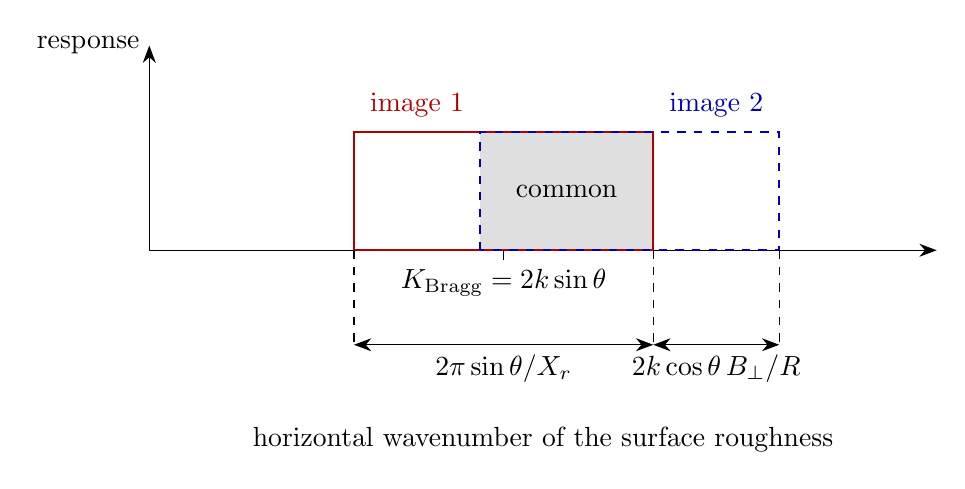
\begin{tikzpicture}[>={Stealth[length=2.2mm]}]
		\draw[->] (0,0) -- (10,0);
		\node at (5,-2.4) {horizontal wavenumber of the surface roughness};
		\draw[->] (0,0) -- (0,2.6) node[left] {response};
		\fill[gray!25] (4.2,0) rectangle (6.4,1.5);
		\draw[thick, red!70!black] (2.6,0) rectangle (6.4,1.5);
		\draw[thick, blue!70!black, dashed] (4.2,0) rectangle (8.0,1.5);
		\node[red!70!black] at (3.4,1.85) {image 1};
		\node[blue!70!black] at (7.2,1.85) {image 2};
		\node at (5.3,0.75) {common};
		\draw (4.5,0) -- (4.5,-0.12) node[below] {$K_\mathrm{Bragg} = 2k\sin\theta$};
		\draw[dashed] (2.6,0) -- (2.6,-1.25);
		\draw[dashed] (6.4,0) -- (6.4,-1.25);
		\draw[dashed] (8.0,0) -- (8.0,-1.25);
		\draw[<->] (2.6,-1.2) -- node[below] {$2\pi\sin\theta/X_r$} (6.4,-1.2);
		\draw[<->] (6.4,-1.2) -- node[below] {$2k\cos\theta\,\Bperp/R$} (8.0,-1.2);
	\end{tikzpicture}
	\caption{The physics of spatial (baseline) decorrelation. Each image responds to a band of surface-roughness wavenumbers centered on the Bragg wavenumber (Lecture 8), with a width set by the range resolution. The two look angles shift the bands relative to each other; only the common part (gray) contributes to the coherence, and the coherence vanishes at the critical baseline, when the shift equals the band width.}
	\label{f:wavenumber}
\end{figure}

\subsection{Volume decorrelation}

\begin{itemize}
	\item For a surface scatterer, all of the scattering in a resolution cell comes from (nearly) the same height. In a volume (vegetation, snow, ice, dry sand; Lecture 9), the scatterers are distributed over a range of heights
	\item By Eq.~\eqref{e:topo}, scatterers at different heights $z$ in the same resolution cell have different interferometric phases, $-k_zz$, where the \emph{vertical wavenumber} is
	\begin{equation}
		\label{e:kz}
		k_z = \frac{4\pi\Bperp}{\lambda R\sin\theta} = \frac{2\pi}{\zamb}
	\end{equation}
	The sum over the volume of phasors with different phases has a magnitude less than one: \emph{volume decorrelation}
	\item Model: a layer of thickness $d$ (e.g., a forest canopy) with uniform scatterers and extinction coefficient $\kappa_\mathrm{e}$ (Lecture 9), over a ground that we neglect for now. Power scattered at height $z$ above the bottom of the layer is attenuated on the way in and out by $e^{-2\kappa_\mathrm{e}(d - z)/\cos\theta}$, so
	\begin{equation}
		\label{e:gvol}
		\gt_\mathrm{vol} = \frac{\int_0^d e^{2\kappa_\mathrm{e}z/\cos\theta}\,e^{-jk_zz}\,dz}{\int_0^d e^{2\kappa_\mathrm{e}z/\cos\theta}\,dz}
	\end{equation}
	% NOTE: Rosen et al. (2000), Eqs. 63-64: gamma_Z = int f(z) exp(-j kappa_z z) dz with f the normalized effective
	% scatterer profile; here f is the exponential profile of a uniform random volume (Treuhaft and Siqueira, 2000);
	% the weighting follows
	% the two-way canopy transmissivity of L9 (Upsilon^2 = e^{-2 kappa_e d/cos theta}). Closed form (python3/sympy):
	% gamma_vol = p (e^{(p - j k_z) d} - 1)/((p - j k_z)(e^{p d} - 1)), p = 2 kappa_e/cos(theta).
	\begin{itemize}
		\item Transparent layer ($\kappa_\mathrm{e} \to 0$): $\gamma_\mathrm{vol} = |\sin(k_zd/2)/(k_zd/2)|$, which drops to zero when $d = \zamb$
		\item Strong extinction: only the top of the layer is seen, the effective thickness is $\sim$$\cos\theta/(2\kappa_\mathrm{e})$, and $\gamma_\mathrm{vol} \to 1$
		\item The phase of $\gt_\mathrm{vol}$ places the effective scattering center between the ground and the top of the canopy. Longer waves are scattered less by leaves and twigs and penetrate deeper, so the scattering center is lower at L-band than at C-band, and DEMs from C-band InSAR over forests sit closer to the canopy top (Rosen et al., 2000, p.~354)
	\end{itemize}
	\item[$\Rightarrow$] Volume decorrelation is not just a nuisance: with the ground term added (Lecture 9 again) and several baselines or polarizations, it is used to estimate forest height (polarimetric InSAR; Treuhaft and Siqueira, 2000)
\end{itemize}

\subsection{Temporal decorrelation}

\begin{itemize}
	\item In repeat-pass interferometry, the scatterers themselves change between $t_1$ and $t_2$. Any change in their positions or properties that differs within a resolution cell randomizes the phase
	\item Zebker and Villasenor (1992) model random motion of the scatterers, with rms displacements $\Delta y_\mathrm{rms}$ (horizontal, in the range direction) and $\Delta z_\mathrm{rms}$ (vertical). Each scatterer's phase changes by $(4\pi/\lambda)$ times its displacement along the line of sight, and for Gaussian displacements
	\begin{equation}
		\label{e:gtemp}
		\gamma_\mathrm{temporal} = \exp\left[-\frac12\left(\frac{4\pi}{\lambda}\right)^2\left(\Delta y_\mathrm{rms}^2\sin^2\theta + \Delta z_\mathrm{rms}^2\cos^2\theta\right)\right]
	\end{equation}
	% NOTE: Zebker and Villasenor (1992), Eq. 24 (p. 954; their sigma_y, sigma_z renamed; sigma is taken in the master
	% table). Their Fig. 4: complete decorrelation at ~10 cm rms motion at L-band, 2-3 cm at C-band.
	% Derivation: <exp(j Delta phi_n)> = exp(-<Delta phi_n^2>/2) for zero-mean Gaussian Delta phi_n.
	\begin{itemize}
		\item $\gamma_\mathrm{temporal} = 0.5$ for $\Delta z_\mathrm{rms}\cos\theta \approx 0.09\lambda$: at $\theta = 37^\circ$, about 6.5~mm at C-band but 2.8~cm at L-band (Figure~\ref{f:gtemp})
		% NOTE: python3: sqrt(2 ln 2) lambda/(4 pi) = 0.0937 lambda; divided by cos(37 deg): 6.5 mm (C, lambda = 5.55 cm),
		% 28 mm (L, 23.8 cm).
		\item[$\Rightarrow$] Longer wavelengths tolerate more random motion: L-band stays coherent over vegetation and through seasons where C-band does not
	\end{itemize}
	\item Physical causes, connecting to earlier lectures:
	\begin{itemize}
		\item Vegetation: wind moves leaves and branches; growth and harvest (Lecture 9)
		\item Changes in $\varepsilon$: wetting and drying of soil, freezing and thawing (Lecture 1)
		\item Snow: accumulation, melt, and changes in the snowpack (Lectures 1, 9)
		\item Water: the ocean surface moves continuously (Lecture 8) and decorrelates in much less than a second, far faster than any repeat cycle
		\item Wind-blown sand: in a C-band interferogram of the Algodones Dunefield (California), active, unvegetated dunes stayed correlated over one day but decorrelated completely over five months, while partially vegetated dunes stayed correlated (Rosen et al., 2000, p.~351 and Fig.~23)
		% NOTE: Rosen et al. (2000), p. 351: "active, unvegetated dunes completely decorrelate after five months (though
		% not in one day), but ... partially vegetated dunes remain correlated" (ERS-1/2, C-band).
		\item Disturbance: fire, flooding, landslides, construction, and earthquake ruptures rearrange the scatterers
	\end{itemize}
	\item[$\Rightarrow$] Loss of coherence is itself a signal. For example, maps of coherence loss are used to map the damage from earthquakes, floods, and fires; it complements the change in backscatter that we used to map the Eaton Fire in Problem Set 3
\end{itemize}

\begin{figure}[!htbp]
	\centering
	% NOTE: plotted from Eq. (e:gtemp) with Delta y_rms = 0 and theta = 37 deg; lambda = 5.55 cm (C) and 23.8 cm (L).
	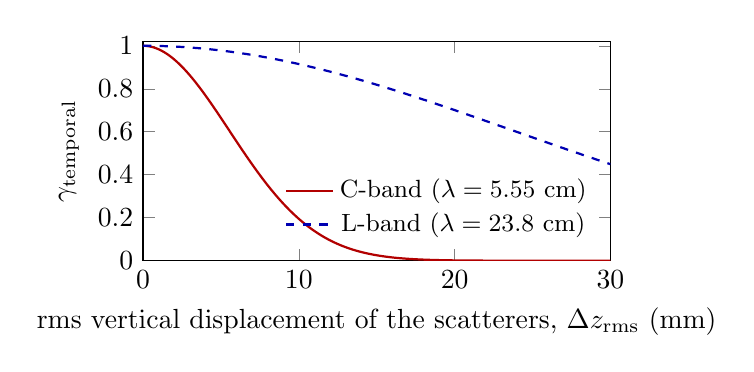
\begin{tikzpicture}
		\begin{axis}[
			width=0.62\textwidth, height=0.36\textwidth,
			xmin=0, xmax=30, ymin=0, ymax=1.02,
			xlabel={rms vertical displacement of the scatterers, $\Delta z_\mathrm{rms}$ (mm)},
			ylabel={$\gamma_\mathrm{temporal}$},
			legend style={at={(0.98,0.06)}, anchor=south east, draw=none, fill=none, font=\small},
			samples=150, domain=0:30]
			\addplot[thick, red!70!black] {exp(-0.5*(4*pi/55.5)^2*(x*cos(37))^2)};
			\addlegendentry{C-band ($\lambda = 5.55$~cm)}
			\addplot[thick, blue!70!black, dashed] {exp(-0.5*(4*pi/238)^2*(x*cos(37))^2)};
			\addlegendentry{L-band ($\lambda = 23.8$~cm)}
		\end{axis}
	\end{tikzpicture}
	\caption{Temporal decorrelation from random vertical motion of the scatterers, Eq.~\eqref{e:gtemp}, for a look angle of $37^\circ$. Random motion of about a centimeter destroys the coherence at C-band but only modestly reduces it at L-band.}
	\label{f:gtemp}
\end{figure}

%%%%%%%%%%%%%%%%%%%%%%%%%%%%%%%%%%%%%
\section{Propagation delays}
\label{s:delay}

\begin{itemize}
	\item So far we have assumed that the wave travels at $c$. In the atmosphere it travels at $u_p = c/n'$ (Lecture 2: $c/\sqrt{\varepsilon'}$), with $n'$ slightly different from 1, so the phase measures an \emph{effective} (electrical) path length
	\item The excess one-way path length is $\Delta R_\mathrm{atm} = \int(n' - 1)\,dR$ along the ray, and it adds to $R$ in Eq.~\eqref{e:phi}. The interferogram sees the \emph{difference} between the delays at $t_1$ and $t_2$:
	\begin{equation}
		\label{e:datm}
		\Delta\phi_\mathrm{atm} = \frac{4\pi}{\lambda}\left[\Delta R_\mathrm{atm}(t_2) - \Delta R_\mathrm{atm}(t_1)\right]
	\end{equation}
	\item Two parts of the atmosphere matter: the neutral troposphere and the ionosphere (Lecture 10)
\end{itemize}

\subsection{Refractivity of the neutral atmosphere}

\begin{itemize}
	\item Because $n' - 1$ is tiny, it is written as the \emph{refractivity} $N = 10^6(n' - 1)$. For the neutral atmosphere at microwave frequencies (Hanssen 2001, Eqs.~6.1.7--6.1.9; Smith and Weintraub, 1953)
	\begin{equation}
		\label{e:N}
		N = k_1\frac{\Pdry}{T} + k_2\frac{\Pvap}{T} + k_3\frac{\Pvap}{T^2} \approx k_1\frac{P}{T} + k_3\frac{\Pvap}{T^2}
	\end{equation}
	% NOTE: Hanssen (2001), Eq. 6.1.7 (p. 202) and Eq. 6.1.8; his P_d and e are written P_dry and P_vap. Writing the
	% first term with the total pressure P moves (k_2 - k_1) P_vap/T into the vapor terms; Hanssen's Eq. 6.1.8 uses
	% k_2' = 23.3 K/hPa (Eq. 6.1.9), which applies with the virtual temperature (his footnote 1). Either way this term is
	% <~2% of the wet refractivity at 270 K (python3), so it is dropped here.
	\begin{itemize}
		\item[] $\Pdry$, $\Pvap$: partial pressures of dry air and water vapor, $P = \Pdry + \Pvap$; $T$ in K
		\item[] $k_1 = 77.6$~K/hPa, $k_2 = 71.6$~K/hPa, $k_3 = 3.75\times10^5$~K$^2$/hPa (values as used by Hanssen, 2001, p.~202), with pressures in hPa. In SI units (pressures in Pa), $k_1 = 0.776$~K/Pa and $k_3 = 3.75\times10^3$~K$^2$/Pa, which we use below
		\item First term: induced dipoles of all molecules (\emph{hydrostatic} term). Second and third: water vapor, whose permanent dipole moment (Lecture 1) gives the large $k_3$ term (\emph{wet} term)
	\end{itemize}
	\item $N$ does not depend on frequency at microwave frequencies away from the rotational absorption lines of H$_2$O (22~GHz) and O$_2$ (60~GHz) (Lecture 11): the troposphere is \emph{non-dispersive} for radar
	\item At sea level, $N \approx 270$ for dry air ($n' - 1 \approx 2.7\times10^{-4}$), and the wet term adds up to $\sim$$150$ in warm, saturated air
	% NOTE: python3: 77.6 * 1013/288 = 273; saturated air: 134 at 25 C, 173 at 30 C (reviewer check).
\end{itemize}

\subsection{Hydrostatic and wet delays}

\begin{itemize}
	\item \emph{Hydrostatic delay.} Using the ideal gas law $P = \rho_\mathrm{air}R_\mathrm{gas}T/M$ (here $\rho_\mathrm{air}$ is the density of moist air; the difference from dry air is $<1\%$), the first term of Eq.~\eqref{e:N} is $k_1\rho_\mathrm{air}R_\mathrm{gas}/M$, and the zenith delay from the surface (elevation $z_s$) up is
	\begin{equation}
		\label{e:zhd}
		\Delta R^\mathrm{zen}_\mathrm{hyd} = 10^{-6}k_1\frac{R_\mathrm{gas}}{M}\int_{z_s}^\infty\rho_\mathrm{air}\,dz = 10^{-6}k_1\frac{R_\mathrm{gas}}{Mg}P_s
	\end{equation}
	% NOTE: Hanssen (2001), Eqs. 6.1.10-6.1.13 (p. 203), with R_d = R_gas/M; hydrostatic balance P_s = g int rho dz
	% (L10). python3: 2.31 m for P_s = 1013.25 hPa (k_1 = 0.776 K/Pa, g = 9.784, Hanssen's column-mean gravity g_m,
	% Eq. 6.1.12); Hanssen: 2.3 m. Hanssen's footnote 1 (p. 202): strictly, the virtual temperature (moist air).
	\begin{itemize}
		\item Only the surface pressure $P_s$ matters, by hydrostatic balance (Lecture 10)! With $P_s$ in Pa, $\Delta R^\mathrm{zen}_\mathrm{hyd} \approx 2.3$~m at sea level, or 2.3~mm per hPa
		\item Large but smooth: surface pressure usually varies by less than 1~hPa over 100~km (Hanssen, 2001, Sec.~6.1.3), so over flat terrain the hydrostatic delay adds only a nearly uniform offset or a gentle ramp to an interferogram. Over topography it does not cancel completely (Eq.~\eqref{e:strat} below)
	\end{itemize}
	\item \emph{Wet delay.} With $\Pvap = \rho_\mathrm{vap}R_\mathrm{gas}T/\Mvap$, the wet term is $k_3R_\mathrm{gas}\rho_\mathrm{vap}/(\Mvap T)$, and
	\begin{equation}
		\label{e:zwd}
		\Delta R^\mathrm{zen}_\mathrm{wet} \approx 10^{-6}\frac{k_3R_\mathrm{gas}}{\Mvap T_m}\int_{z_s}^\infty\rho_\mathrm{vap}\,dz = 10^{-6}\frac{k_3R_\mathrm{gas}}{\Mvap T_m}\,\wv
	\end{equation}
	% NOTE: derived from Eq. (e:N); T_m is a vapor-weighted mean temperature of the column. python3 with k_3 = 3750
	% K^2/Pa, R_gas/M_vap = 461.5 J/(kg K): 6.6, 6.4, 6.2 mm of delay per kg/m^2 for T_m = 260, 270, 280 K;
	% 6.4 * 50 = 320 mm. Hanssen (2001, p. 203, citing Elgered 1982) gives a wet delay of less than ~0.3 m for his
	% (mid-latitude) test sites.
	where $\wv$ is the column water vapor (mass per unit area; 1~kg/m$^2$ is 1~mm of liquid water) and $T_m \approx 270$~K is a mean temperature of the column
	\begin{itemize}
		\item[$\Rightarrow$] $\Delta R^\mathrm{zen}_\mathrm{wet} \approx 6.4\,\wv$ (both in mm of length): the wet delay is about six times the depth of the condensed water
		\item Standard atmosphere ($\rho_{\mathrm{vap},0} = 7.72$~g/m$^3$, $H_\mathrm{vap} = 2$~km, so $\wv = \rho_{\mathrm{vap},0}H_\mathrm{vap} \approx 15$~kg/m$^2$): $\Delta R^\mathrm{zen}_\mathrm{wet} \approx 10$~cm. Very humid air with $\wv \approx 50$~kg/m$^2$: $\approx 30$~cm
		% NOTE: python3: 6.4 * 15.4 = 99 mm.
		\item Smaller than the hydrostatic delay, but highly variable in space and time, because water vapor is (Lecture 10)
	\end{itemize}
	\item In the interferogram, both delays are multiplied by $\approx 1/\cos\theta$ to map them to the slant path
\end{itemize}

\subsection{Stratified and turbulent delays}

\begin{itemize}
	\item \emph{Stratified delay.} The delay to a pixel is the integral from the pixel's elevation upward, so it decreases with elevation. With the exponential profiles of Lecture 10,
	\begin{equation}
		\label{e:strat}
		\Delta R^\mathrm{zen}_\mathrm{hyd}(z) \propto e^{-z/H_p}, \qquad \Delta R^\mathrm{zen}_\mathrm{wet}(z) \propto e^{-z/H_\mathrm{vap}}
	\end{equation}
	\begin{itemize}
		\item If the atmosphere differs between $t_1$ and $t_2$, the interferogram contains a phase that correlates with topography, which can be mistaken for deformation (e.g., inflation of a volcano)
		\item Example: a 30\% change in $\rho_{\mathrm{vap},0}$ between acquisitions over terrain from 0 to 2~km ($H_\mathrm{vap} = 2$~km): the change in zenith wet delay is 3.0~cm at sea level but 1.1~cm at 2~km, a difference of 1.9~cm, or 2.4~cm along a slant path at $37^\circ$: almost one fringe at C-band
		% NOTE: python3: 0.3 * 9.9 cm = 3.0 cm; 3.0 e^{-1} = 1.1 cm; 1.9/cos(37 deg) = 2.4 cm; lambda/2 = 2.8 cm.
		\item This is exactly the measurement you made from space in Problem Set 3: the scale height $H_\mathrm{vap}$ tells you how fast the wet delay falls with elevation
	\end{itemize}
	\item \emph{Turbulent delay.} Turbulent mixing in the boundary layer makes the water vapor patchy on scales of $\sim$1 to tens of km, independent of topography. The resulting delay differences grow with the distance $L$ between points: from GPS in southern California, the standard deviation of the change in (one-way, zenith) delay difference between two times is about $2.5\sqrt{L/\mathrm{1~km}}$~mm, or 8~mm at 10~km and 25~mm at 100~km (Emardson et al., 2003)
	% NOTE: Emardson et al. (2003), Eq. 5 (p. ETG 4-3): sigma = c L^alpha + k H, the std of the two-epoch difference of
	% the one-way zenith delay difference between two points (from SCIGN GPS); they adopt c = 2.5 mm, alpha = 0.5 (L in km)
	% and neglect the H term (k = 4.8 mm/km in their Table 1). python3: 7.9 mm at 10 km, 25 mm at 100 km.
	\item Mitigation: weather models (e.g., ERA5), GNSS zenith delays, the correlation with topography, and averaging many interferograms (the turbulent part is random in time)
\end{itemize}

\subsection{The ionosphere}

\begin{itemize}
	\item The ionosphere ($\sim$60--1000~km altitude) contains free electrons, with number density $N_\mathrm{e}$ up to $\sim$$10^{12}$~m$^{-3}$
	\item Free electrons are an oscillator with no restoring force (Lecture 1, with $\omega_0 = 0$; Lecture 10 introduced the ionosphere and its dispersion), so, without collisions, $\varepsilon = 1 - \omega_p^2/\omega^2$ with the plasma frequency $\omega_p^2 = N_\mathrm{e}e^2/(\varepsilon_0m_\mathrm{e})$. For $\omega \gg \omega_p$,
	\begin{equation}
		\label{e:niono}
		n = \sqrt{\varepsilon} \approx 1 - \frac{\omega_p^2}{2\omega^2} = 1 - \frac{e^2}{8\pi^2\varepsilon_0m_\mathrm{e}}\frac{N_\mathrm{e}}{f^2} \approx 1 - 40.3\,\frac{N_\mathrm{e}}{f^2}
	\end{equation}
	% NOTE: python3: e^2/(8 pi^2 eps_0 m_e) = 40.31 m^3/s^2; Hanssen (2001), Eq. 6.3.4 (p. 211) gives K = -40.28 m^3 s^-2.
	% Plasma frequency for N_e = 1e12 m^-3: f_p = 9 MHz << radar frequencies.
	\item $n < 1$: the phase velocity exceeds $c$, and the phase is \emph{advanced} (the group, which carries the pulse envelope, is delayed by the same amount; Lecture 11, $u_g$). The excess phase path is
	\begin{equation}
		\label{e:diono}
		\Delta R_\mathrm{iono} = -40.3\,\frac{\TEC}{f^2}, \qquad \TEC = \int N_\mathrm{e}\,dR
	\end{equation}
	where the total electron content TEC is measured in TEC units (1~TECU $= 10^{16}$~electrons/m$^2$; typical vertical TEC is 5--50~TECU, more at solar maximum)
	% NOTE: Hanssen (2001), Eq. 6.3.4 and p. 209 (TECU) and p. 211 (0-100 TECU range).
	\item[$\bigstar$] The ionosphere is \emph{dispersive}: the delay scales as $1/f^2$. A change of 1~TECU between acquisitions changes the one-way path by 1.4~cm at C-band (half a fringe) but 25~cm at L-band (two fringes)
	% NOTE: python3: 40.3e16/(5.405e9)^2 = 1.38 cm; 40.3e16/(1.257e9)^2 = 25.5 cm; fringes = 2 Delta R/lambda: 0.50 (C),
	% 2.14 (L). Hanssen (2001), Eq. 6.3.6: -0.015 m per TECU at 5.3 GHz and 23 deg incidence, about half a cycle.
	\begin{itemize}
		\item In terms of apparent displacement, L-band is $(5.405/1.257)^2 \approx 18$ times more sensitive to the ionosphere than C-band; in terms of phase (radians), $5.405/1.257 \approx 4.3$ times
		\item Ionospheric variations over long distances (orbit-like ramps) are largely absorbed with orbit errors; short-wavelength structure (e.g., near the equator and the poles) can dominate L-band interferograms
	\end{itemize}
	\item Every non-dispersive term (troposphere, topography, deformation) gives a phase $\propto f$, while the ionospheric phase $\propto 1/f$, so measuring the phase in two parts of the radar band (\emph{split-spectrum}) separates the ionosphere from everything else
\end{itemize}

%%%%%%%%%%%%%%%%%%%%%%%%%%%%%%%%%%%%%
\section{Choosing a wavelength}
\label{s:wavelength}

Most of the physics above depends on the wavelength. Table~\ref{t:wavelength} compares C-band (Sentinel-1) and L-band (NISAR) for the same geometry.

\begin{table}[!htbp]
	\centering
	\small
	% NOTE: python3, R = 880 km, theta = 37 deg, B_perp = 100 m; X_r = 2.7 m (Sentinel-1 IW) for both, for comparison;
	% Delta z for gamma_temporal = 0.5 with theta = 37 deg.
	\begin{tabular}{l c c c}
		\hline
		& Scaling & C-band (5.405 GHz) & L-band (1.257 GHz) \\
		\hline
		Wavelength $\lambda$ & -- & 5.55~cm & 23.8~cm \\
		Range change per fringe, $\lambda/2$ & $\lambda$ & 2.8~cm & 11.9~cm \\
		Height of ambiguity, $\Bperp = 100$~m & $\lambda$ & 150~m & 630~m \\
		Critical baseline, $X_r = 2.7$~m & $\lambda$ & 7~km & 29~km \\
		Vertical random motion for $\gamma_\mathrm{temporal} = 0.5$ & $\lambda$ & 6.5~mm & 28~mm \\
		Ionospheric path per TECU & $\lambda^2$ & 1.4~cm & 25~cm \\
		Penetration into vegetation, soil, snow & increases with $\lambda$ & shallower & deeper \\
		\hline
	\end{tabular}
	\caption{How the wavelength sets what InSAR measures. The same phase precision gives finer range precision at shorter wavelengths, but longer wavelengths keep their coherence over vegetation and through time.}
	\label{t:wavelength}
\end{table}

\begin{itemize}
	\item C-band: more phase per millimeter of motion, weaker ionospheric effects, but loses coherence quickly over vegetation, snow, and agricultural land
	\item L-band: coherent over longer times and penetrates deeper into vegetation, soil, and snow (Lecture 2: for a given $\varepsilon''$, $\delta_p$ grows with $\lambda$), but less phase per millimeter of motion and much more sensitive to the ionosphere
	\item X-band (3~cm): most sensitive to motion and usually allocated the widest bandwidths (finest resolution), but decorrelates fastest
	\item[$\Rightarrow$] The choice of wavelength is a choice of which physics you want to see and which you want to avoid
\end{itemize}

%%%%%%%%%%%%%%%%%%%%%%%%%%%%%%%%%%%%%
% NOTE: all entries with a DOI checked against their Crossref records (2026-11-19); Gatelli: Crossref misspells
% "Guarnieri". The Treatise chapter is the 2007 first edition (the copy in the instructor's Zotero library).
\section*{References}

{\raggedright
\begin{list}{}{\leftmargin=1.5em \itemindent=-1.5em \itemsep=4pt}
	\item Emardson, T.~R., Simons, M., and Webb, F.~H. (2003). Neutral atmospheric delay in interferometric synthetic aperture radar applications: Statistical description and mitigation. \textit{Journal of Geophysical Research: Solid Earth}, 108(B5), 2231. doi:10.1029/2002JB001781.
	\item Gatelli, F., Monti Guarnieri, A., Parizzi, F., Pasquali, P., Prati, C., and Rocca, F. (1994). The wavenumber shift in SAR interferometry. \textit{IEEE Transactions on Geoscience and Remote Sensing}, 32(4), 855--865. doi:10.1109/36.298013.
	\item Hanssen, R.~F. (2001). \textit{Radar Interferometry: Data Interpretation and Error Analysis}. Dordrecht: Kluwer Academic Publishers. doi:10.1007/0-306-47633-9.
	\item Nolan, M., Fatland, D.~R., and Hinzman, L. (2003). DInSAR measurement of soil moisture. \textit{IEEE Transactions on Geoscience and Remote Sensing}, 41(12), 2802--2813. doi:10.1109/TGRS.2003.817211.
	\item Massonnet, D., Rossi, M., Carmona, C., Adragna, F., Peltzer, G., Feigl, K., and Rabaute, T. (1993). The displacement field of the Landers earthquake mapped by radar interferometry. \textit{Nature}, 364(6433), 138--142. doi:10.1038/364138a0.
	\item Rodr\'iguez, E., and Martin, J.~M. (1992). Theory and design of interferometric synthetic aperture radars. \textit{IEE Proceedings F (Radar and Signal Processing)}, 139(2), 147--159. doi:10.1049/ip-f-2.1992.0018.
	\item Rosen, P.~A., Hensley, S., Joughin, I.~R., Li, F.~K., Madsen, S.~N., Rodr\'iguez, E., and Goldstein, R.~M. (2000). Synthetic aperture radar interferometry. \textit{Proceedings of the IEEE}, 88(3), 333--382. doi:10.1109/5.838084.
	\item Simons, M., and Rosen, P.~A. (2007). Interferometric synthetic aperture radar geodesy. In T.~A. Herring (Ed.), \textit{Treatise on Geophysics} (Vol.~3, Geodesy, pp.~391--446). Amsterdam: Elsevier. doi:10.1016/B978-044452748-6.00059-6.
	\item Smith, E.~K., and Weintraub, S. (1953). The constants in the equation for atmospheric refractive index at radio frequencies. \textit{Proceedings of the IRE}, 41(8), 1035--1037. doi:10.1109/JRPROC.1953.274297.
	\item Treuhaft, R.~N., and Siqueira, P.~R. (2000). Vertical structure of vegetated land surfaces from interferometric and polarimetric radar. \textit{Radio Science}, 35(1), 141--177. doi:10.1029/1999RS900108.
	\item van Zyl, J.~J. (2011). \textit{Synthetic Aperture Radar Polarimetry}. Hoboken, NJ: Wiley.
	\item Zebker, H.~A., and Villasenor, J. (1992). Decorrelation in interferometric radar echoes. \textit{IEEE Transactions on Geoscience and Remote Sensing}, 30(5), 950--959. doi:10.1109/36.175330.
\end{list}
\par}

%%%%%%%%%%%%%%%%%%%%%%%%%%%%%%%%%%%%%
% Symbols follow the master table in ../variables_master.tex; see it for flagged dual usages.
\clearpage
\section*{Variables}

Units are SI unless stated. Values are given for universal constants and for the examples in the notes (Sentinel-1-like geometry: $R = 880$~km, $\theta = 37^\circ$).

{\small
\renewcommand{\arraystretch}{1.2}
\begin{longtable}{>{$}l<{$} >{\raggedright\arraybackslash}p{0.38\textwidth} >{\raggedright\arraybackslash}p{0.13\textwidth} >{\raggedright\arraybackslash}p{0.22\textwidth}}
\hline
\textrm{Symbol} & Description & Units & Value \\
\hline
\endfirsthead
\hline
\textrm{Symbol} & Description & Units & Value \\
\hline
\endhead
\hline
\endfoot
\multicolumn{4}{l}{\emph{Constants}} \\*
c & speed of light in a vacuum & m/s & $2.998\times10^{8}$ \\
e & elementary charge & C & $1.602\times10^{-19}$ \\
\varepsilon_0 & permittivity of free space & F/m & $8.854\times10^{-12}$ \\
m_\mathrm{e} & electron mass & kg & $9.109\times10^{-31}$ \\
R_\mathrm{gas} & universal gas constant & J\,mol$^{-1}$K$^{-1}$ & $8.314$ \\
j & imaginary unit & -- & $\sqrt{-1}$ \\
\multicolumn{4}{l}{\emph{SAR pixels and interferograms}} \\*
\lambda, f & radar wavelength and frequency & m; Hz & 5.55~cm, 5.405~GHz (C); 23.8~cm, 1.257~GHz (L) \\
R & range to a scatterer; $R_1$, $R_2$ from antennas 1 and 2 & m & 880~km \\
\phi & phase of a SAR pixel ($\phi_1$, $\phi_2$ in images 1 and 2) & rad & $-4\pi R/\lambda$ (point scatterer) \\
V, V_1, V_2 & complex value of a focused SAR pixel (as $V_\mathrm{o}$ in L14); in images 1 and 2 & arb. & -- \\
E_{r(n)}, R_{(n)} & field received from, and range to, scatterer $n$ in a resolution cell & arb.; m & -- \\
\Delta\phi & interferometric phase, $\phi_1 - \phi_2$ (subscripts flat, topo, def, atm, scat, noise: its parts) & rad & -- \\
\Delta R & change in range between images ($\Delta R_\mathrm{def}$: from deformation, positive away from the radar) & m & $\lambda/2$ per fringe \\
\delta R_{2\pi} & spacing of flat-Earth fringes in slant range & m & 184 ($\Bperp = 100$~m, C) \\
t_1, t_2 & times of the first (reference) and second acquisitions & s & -- \\
X_r, X_a & slant-range and azimuth resolutions (L14) & m & $X_r \approx 2.7$ (Sentinel-1) \\
\multicolumn{4}{l}{\emph{Geometry}} \\*
B & baseline, distance between the two antenna positions & m & 10--100s \\
\Bpar, \Bperp & components of the baseline parallel and perpendicular to the look direction & m & -- \\
\theta & look angle (L14); used for the incidence angle $\theta_i$ (equal on a flat Earth) & rad & $37^\circ$ \\
h & altitude of the radar (L14) & m & -- \\
z & height of a scatterer above the reference surface; altitude (L10) & m & -- \\
\zamb & height of ambiguity, $\lambda R\sin\theta/(2\Bperp)$ & m & 150 ($\Bperp = 100$~m, C) \\
\multicolumn{4}{l}{\emph{Coherence}} \\*
\gt, \gamma & complex coherence and its magnitude & dimensionless & 0--1 \\
\gamma_\mathrm{SNR}, \gamma_\mathrm{spatial} & coherence limited by thermal noise; by the baseline & dimensionless & 0--1 \\
\gamma_\mathrm{vol}, \gamma_\mathrm{temporal} & coherence limited by volume scattering ($\gt_\mathrm{vol}$: complex); by changes in time & dimensionless & 0--1 \\
\Nlooks & number of looks (pixels averaged) & dimensionless & -- \\
\mathrm{SNR} & signal-to-noise ratio (L14) & dimensionless & -- \\
\Bc & critical baseline & m & 7~km (C, $X_r = 2.7$~m) \\
K_\mathrm{Bragg}, k & Bragg wavenumber $2k\sin\theta_i$ (L8); radar wavenumber $2\pi/\lambda$ & rad/m & -- \\
k_z & vertical wavenumber of an interferometer, $2\pi/\zamb$ & rad/m & -- \\
d & thickness of a scattering layer (L6, L9) & m & -- \\
\kappa_\mathrm{e} & extinction coefficient (L9) & Np/m & -- \\
\Delta y_\mathrm{rms}, \Delta z_\mathrm{rms} & rms random displacements of the scatterers, horizontal (range direction) and vertical & m & $\Delta z_\mathrm{rms} = 6.5$~mm (C), 28~mm (L) for $\gamma_\mathrm{temporal} = 0.5$ at $37^\circ$ \\
\multicolumn{4}{l}{\emph{Propagation delays}} \\*
n' & (real) index of refraction (L2) & dimensionless & $\approx 1.0003$ (sea level) \\
u_p, u_g & phase and group velocities (L2, L11) & m/s & $c/n'$ \\
N & refractivity, $10^6(n' - 1)$ & dimensionless & $\approx 270$--$420$ (sea level) \\
k_1, k_2, k_3 & refractivity constants (as used by Hanssen, 2001) & K/hPa; K/hPa; K$^2$/hPa & 77.6; 71.6; $3.75\times10^5$ (SI: $k_1 = 0.776$~K/Pa, $k_3 = 3.75\times10^3$~K$^2$/Pa) \\
P, \Pdry, \Pvap & total pressure; partial pressures of dry air and water vapor & Pa (hPa with Hanssen's $k$'s) & -- \\
P_s, z_s & surface pressure; surface elevation & Pa; m & $1.013\times10^5$ (sea level) \\
T, T_m & temperature; mean temperature of the water-vapor column & K & $T_m \approx 270$ \\
\rho_\mathrm{air}, \rho_\mathrm{vap} & densities of air and water vapor (L10) & kg/m$^3$ & $\rho_{\mathrm{vap},0} = 7.72\times10^{-3}$ \\
M, \Mvap & molar masses of dry air (L10) and water & kg/mol & $2.9\times10^{-2}$; $1.8\times10^{-2}$ \\
g & gravitational acceleration (column mean in Eq.~\eqref{e:zhd}) & m/s$^2$ & $9.78$ (Hanssen's $g_m$; 9.81 at the surface) \\
\wv & column water vapor, $\int\rho_\mathrm{vap}\,dz$ & kg/m$^2$ & $\approx 15$ (standard atmosphere) \\
H_p, H_\mathrm{vap} & pressure and water-vapor scale heights (L10) & m & 8.4~km; 2~km \\
\Delta R_\mathrm{atm} & excess one-way path length through the atmosphere, $\int(n'-1)\,dR$ & m & -- \\
\Delta R^\mathrm{zen}_\mathrm{hyd} & hydrostatic zenith delay (excess path length) & m & 2.3 (sea level) \\
\Delta R^\mathrm{zen}_\mathrm{wet} & wet zenith delay (excess path length) & m & $\sim$0.1 \\
\Delta R_\mathrm{iono} & excess phase path through the ionosphere & m & $-1.4$~cm (C), $-25$~cm (L) per TECU \\
N_\mathrm{e} & electron number density & m$^{-3}$ & up to $\sim$$10^{12}$ \\
\omega_p & plasma frequency (L1) & rad/s & -- \\
\TEC & total electron content, $\int N_\mathrm{e}\,dl$ & m$^{-2}$ (TECU: $10^{16}$~m$^{-2}$) & 5--50~TECU \\
\end{longtable}
}

\end{document}
